\documentclass{beamer}
\usetheme{Singapore}
\usepackage[utf8]{inputenc}
\usecolortheme{crane}
\usepackage{graphicx}
\usepackage{iwona}
\usepackage{standalone}
\usepackage{tikz}
\usetikzlibrary{arrows}
\usetikzlibrary{decorations.markings}
\usetikzlibrary{calc}
\usetikzlibrary{shapes,snakes}
\usepackage{hyperref}
\usepackage{listings}

\definecolor{brown}{RGB}{153, 102, 51}
\definecolor{poolgreen}{RGB}{102, 153, 51}

\beamertemplatenavigationsymbolsempty

\title{Snooker, Smoking, and Floating Point Number Arithmetic}
\author{Geraint Palmer}
\date{}

\begin{document}

\frame{\maketitle}

\frame{
  \includestandalone[width=\textwidth]{pool}
}

\frame{
  \begin{center}
    
\includegraphics[width=0.6\textwidth]{smoke}
  \end{center}
}

% Chaos: When the present predicts the future, the approximate present doesn't predict the approximate future

\frame{
  \frametitle{$x_{k+1} = 4 x_k \left(1 - x_k\right)$\\
  $y_{k+1} = x_k + y_k \mod 1$}
  \begin{center}
  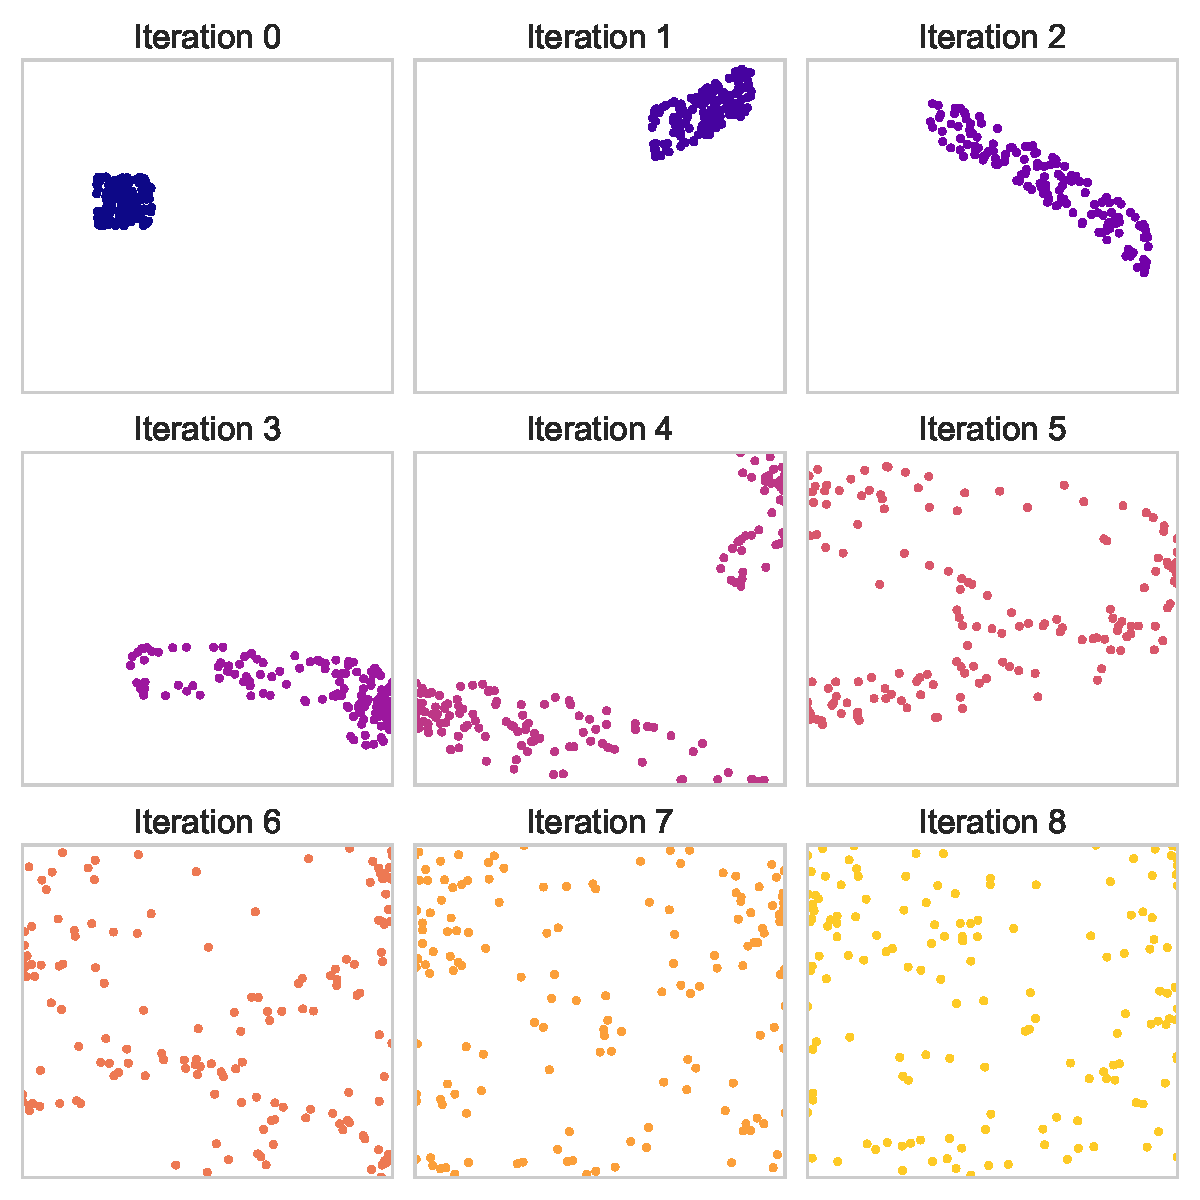
\includegraphics[width=0.6\textwidth]{logistic_map}
  \end{center}
}

\frame{
  \begin{columns}
    \begin{column}{0.4\textwidth}
    \begin{align*}
      \frac{dx}{dt} &= 10(y - x)\\
      \frac{dy}{dt} &= x(28 - z) - y\\
      \frac{dz}{dt} &= xy = \frac{8}{3}z
    \end{align*}
    \end{column}
    \begin{column}{0.6\textwidth}
      \begin{center}
        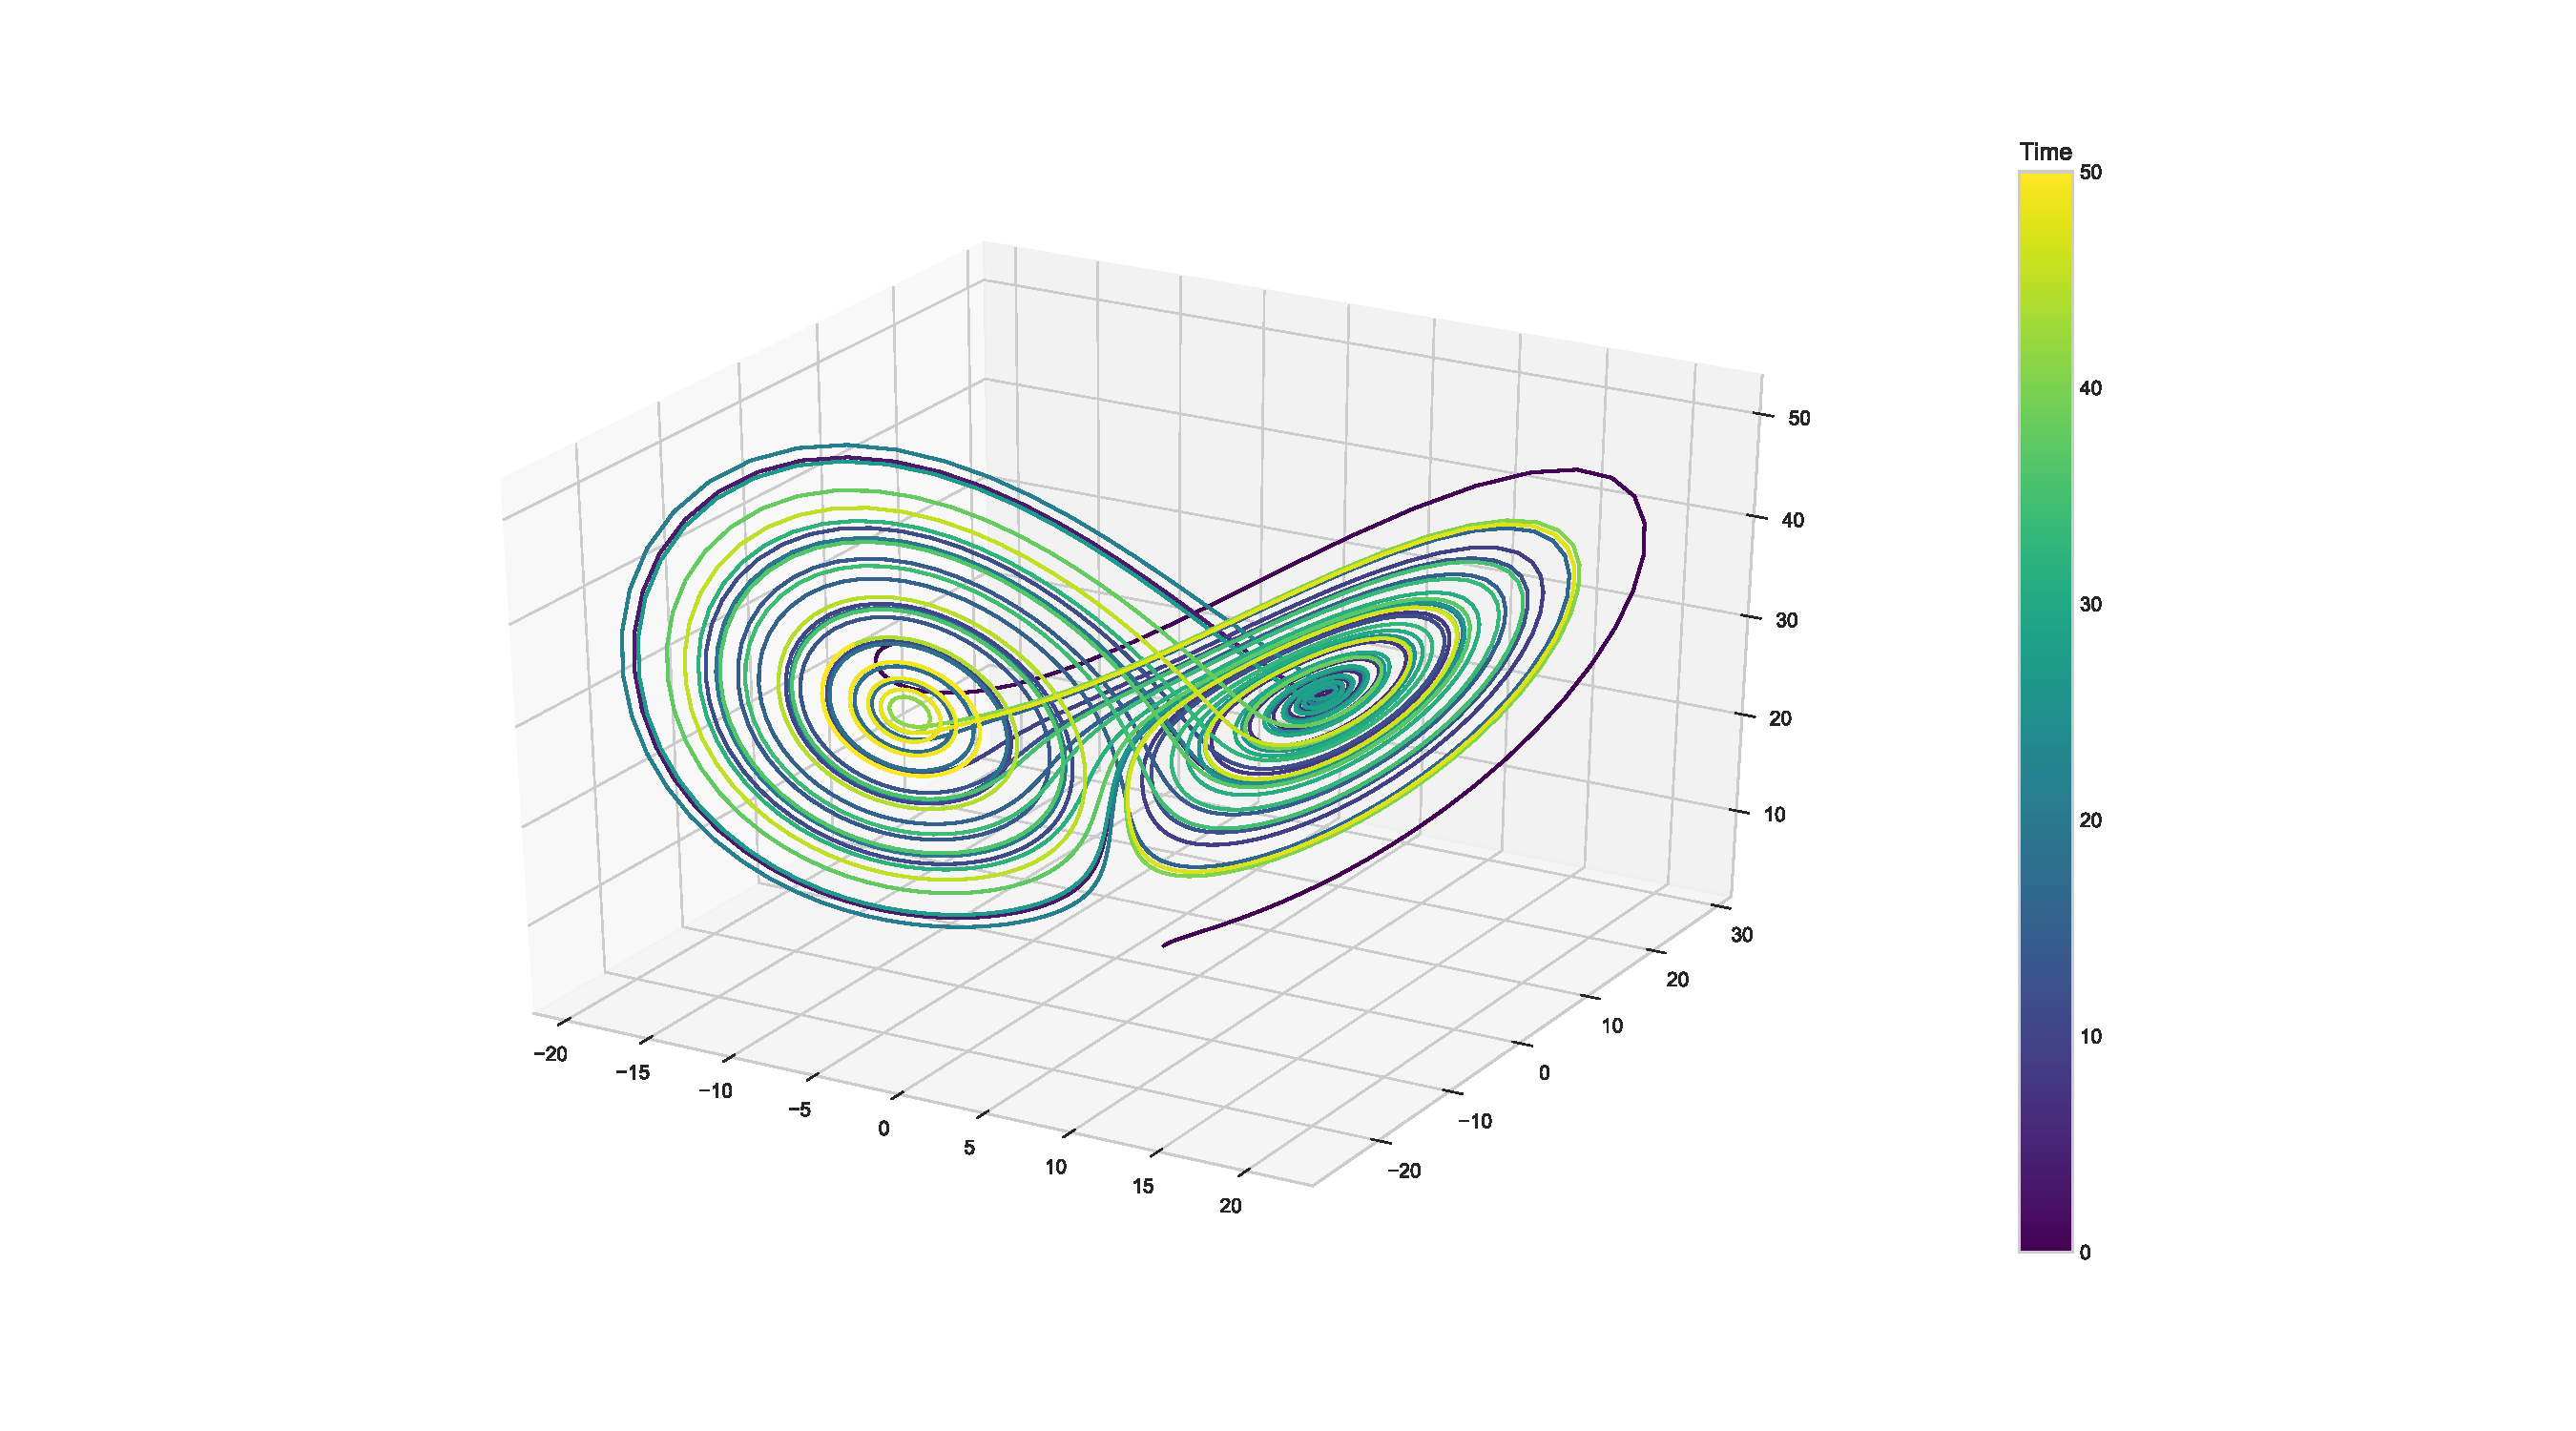
\includegraphics[width=\textwidth]{lorenz}
      \end{center}
    \end{column}
  \end{columns}
}

\frame{
  \begin{center}
  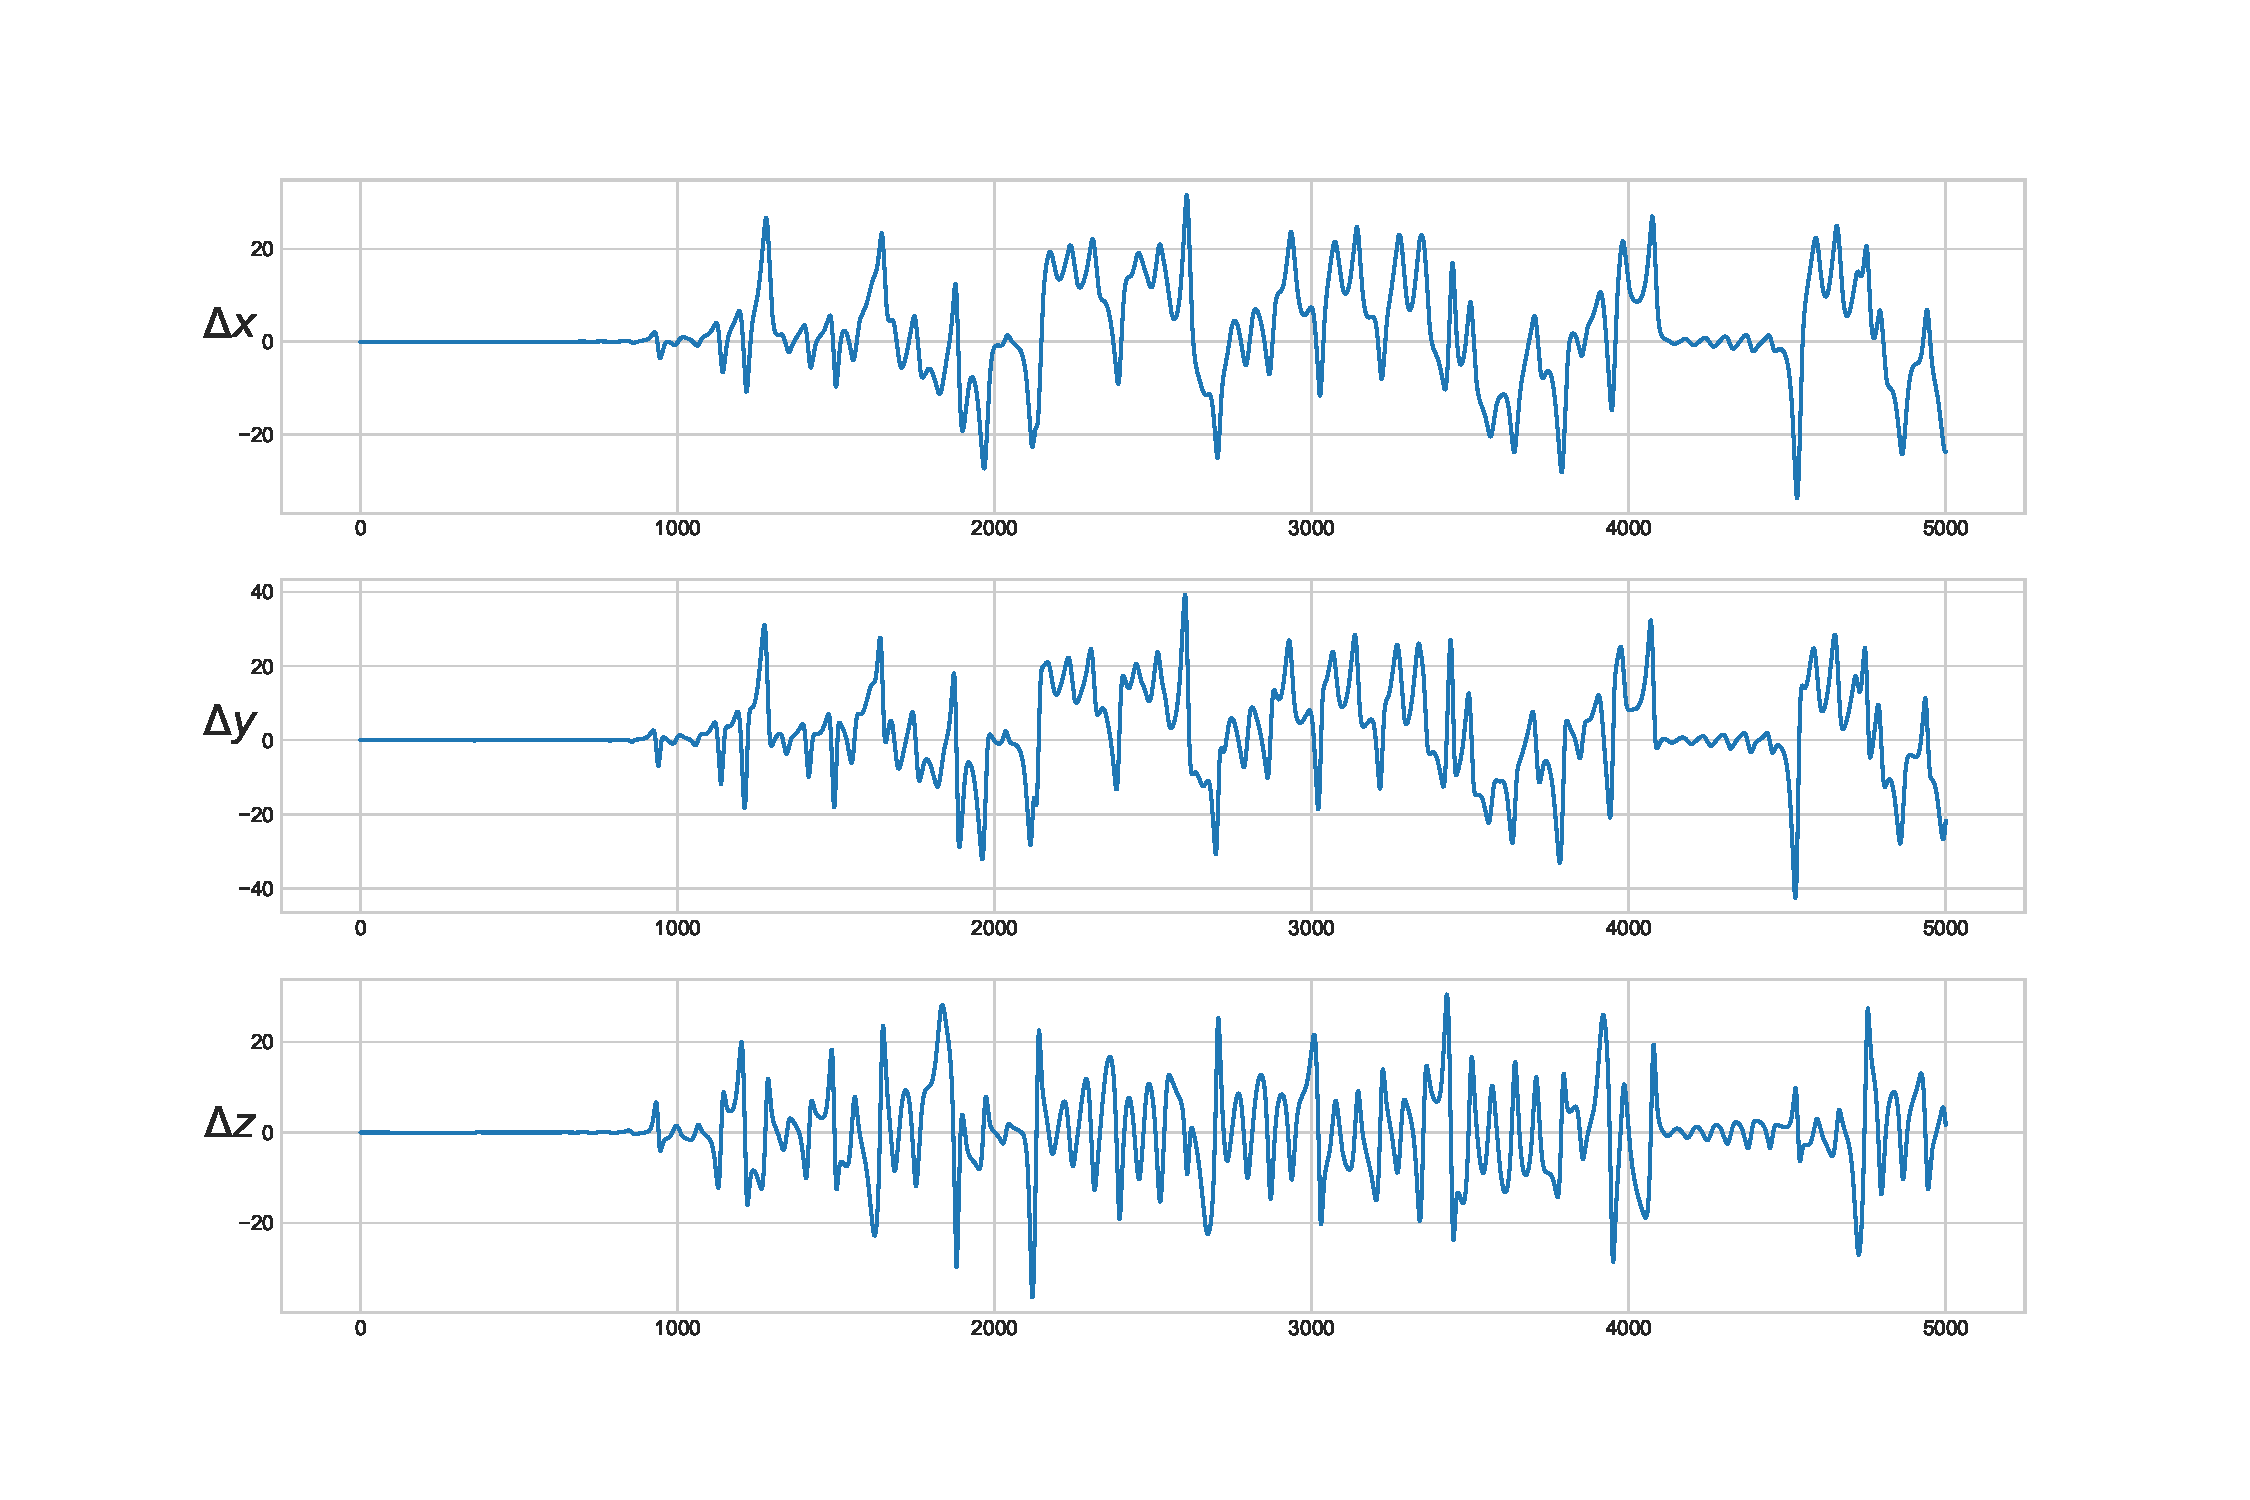
\includegraphics[width=\textwidth]{lorenzediff}
  \end{center}
}

\frame{
  \begin{center}
  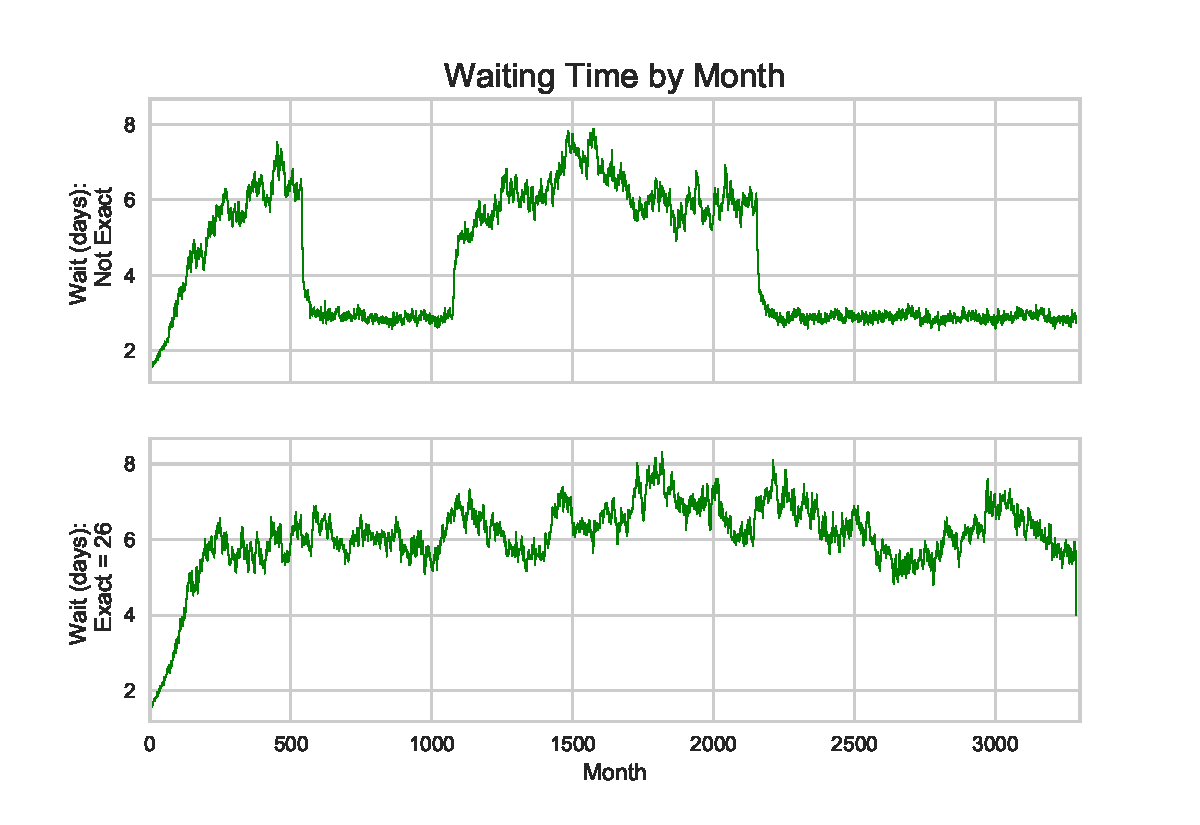
\includegraphics[width=\textwidth]{liekewaits_both}
  \end{center}
}

\begin{frame}[fragile]
\LARGE{
\begin{lstlisting}
>>> 0.1 + 0.2
0.30000000000000004
\end{lstlisting}
}
\end{frame}



\end{document}
